\documentclass[11pt]{article}
\usepackage{physics}
% NOTE: Add in the relevant information to the commands below; or, if you'll be using the same information frequently, add these commands at the top of paolo-pset.tex file. 
\newcommand{\name}{TA: Hossein Mohammadi}
\newcommand{\email}{hossein.mohammadi.00427@gmail.com}
\newcommand{\classnum}{Advanced Quantum Field Theory}
\newcommand{\subject}{Subject: Review of Introductory Course}
\newcommand{\instructors}{Dr. Amin Faraji}
\newcommand{\assignment}{PSet 1}
\newcommand{\semester}{- Fall 1402}
\newcommand{\duedate}{dd/mm/yyyy}

\input{paolo-pset.tex}

% NOTE: To compile a version of this pset without problems, solutions, or reflections, uncomment the relevant line below.

%\excludeversion{problem}
%\excludeversion{solution}
%\excludeversion{reflection}

\begin{document}	
	
	% Use the \psetheader command at the beginning of a pset. 
	\psetheader
	
	\section*{Problem 1: Review of Concepts %\points{50}
	}
	
	\begin{problem}
		In this problem, we will review some concepts which we've encountered with in the Introductory course. Please write you answers clearly and keep your answers as concise as possible.
	\end{problem}
	\begin{enumerate}
		\item
		\begin{problem}{\points[2.3 Peskin]{-}}
			\textbf{Review of Traditional Quantization:}
			
			\noindent
			Consider complex Klein-Gordon model, we quantize this classical model using traditional method, that means expressing fields in terms of ladder operators.
			\begin{enumerate}
				\item Write out the Lagrangian and Hamiltonian of this model, equal-time commutation relation between fields. Describe what helped you to write the commutation relations.
				
				\item  Expand fields in terms of creation-annihilation operators. Work out the commutation relations of ladder operator. By which I mean $[a_\mathbf{p},a^\dagger_\mathbf{q}]$ , $[a_\mathbf{p},a_\mathbf{q}]$ , $[a^\dagger_\mathbf{p},a^\dagger_\mathbf{q}]$.
				
				\item Express Hamiltonian in terms of ladder operators. You need commutation relations in part (ii). Observe that this is nothing but an infinite set of quantum harmonic oscillators.
				
			\end{enumerate}
		\end{problem}
		\item
		\begin{problem}{\points[2.4 Peskin]{-}}
		\textbf{Propagator:}
		
		Propagators (which is nothing but 2 point function), is of crucial importance in perturbative field theory calculation, let's quickly review it.
		\noindent
		\begin{enumerate}
			\item In a free theory, propagator is $\bra{0}T\phi(x)\phi(y)\ket{0}$, so how you can interprete it? what does a propagator mean in physical terms?
			
			\item Describe Feynman prescription for propagator, how it implements the time-ordering within itself?
			
			\item Work out the details of propagator of complex Klein-Gordon model. [ Start from $\bra{0}T\phi(x)\phi(y)\ket{0}$ as Peskin, and implementing the time-ordering, conclude the final form of the propagator which is $D_F(x_1,x_2) = 
			\int \frac{d^4k}{(2\pi)^4} \frac{i}{k^2 -m^2 + i\epsilon} e^{ik.(x_2-x_1)}
			$]
		\end{enumerate}
		\end{problem}
	\item
	\begin{problem}{\points[Peskin Ch3]{-}}
		\textbf{Dirac equation and Spinors:}
		
		\noindent
		Spinor representation of Lorentz group, incorporates electron and all other half-spin integers into the theory. In some senses, spinors are weird, but spin-statistics theorem guarantees its physical significance. Here we just look at some important facts about them.

		\begin{enumerate}
			\item To warm up, write the Clifford algebra, its Dirac and Weyl representation, Lorentz generators of algebra, and finally the dirac equation.
			\item Establish the Lorentz invariance of the dirac equation.[You'll need to know how spinors and $\gamma^\mu$ matrices transform under Lorentz transformation, which could be found in (3.29) and (3.30)]
			\item $[\text{Optional}]$ Repeat the "Problem 1" with spinors, in order to experience manipulations of dirac spinors.
			\item Describe discrete symmetries of Dirac theory: Parity, time reversal and charge conjugation. No need to write any equation at all, just write you understanding of them.
			
		\end{enumerate}
	\end{problem}
	\item
		\begin{problem}{\points[Peskin Ch4]{-}}
			\textbf{Interaction Concepts:}
			
			\noindent
			Perturbative field theory is a understandable framework to work with field theories in special regimes. We review the most important machinaries that was developed to do perturbative field theory.
			\begin{enumerate}
				\item How one finds n-point functions in a field theory? Write out its formula, which is somehow genralization of (4.31). Also write the different stages that we go through during reaching to this equation.
				\item Express and give a minimal example of Wick theorem.
				\item Argue why disconnected diagrams, like the below ones, would not contribute to n-point functions?
				\begin{figure}[h]
					\centering
					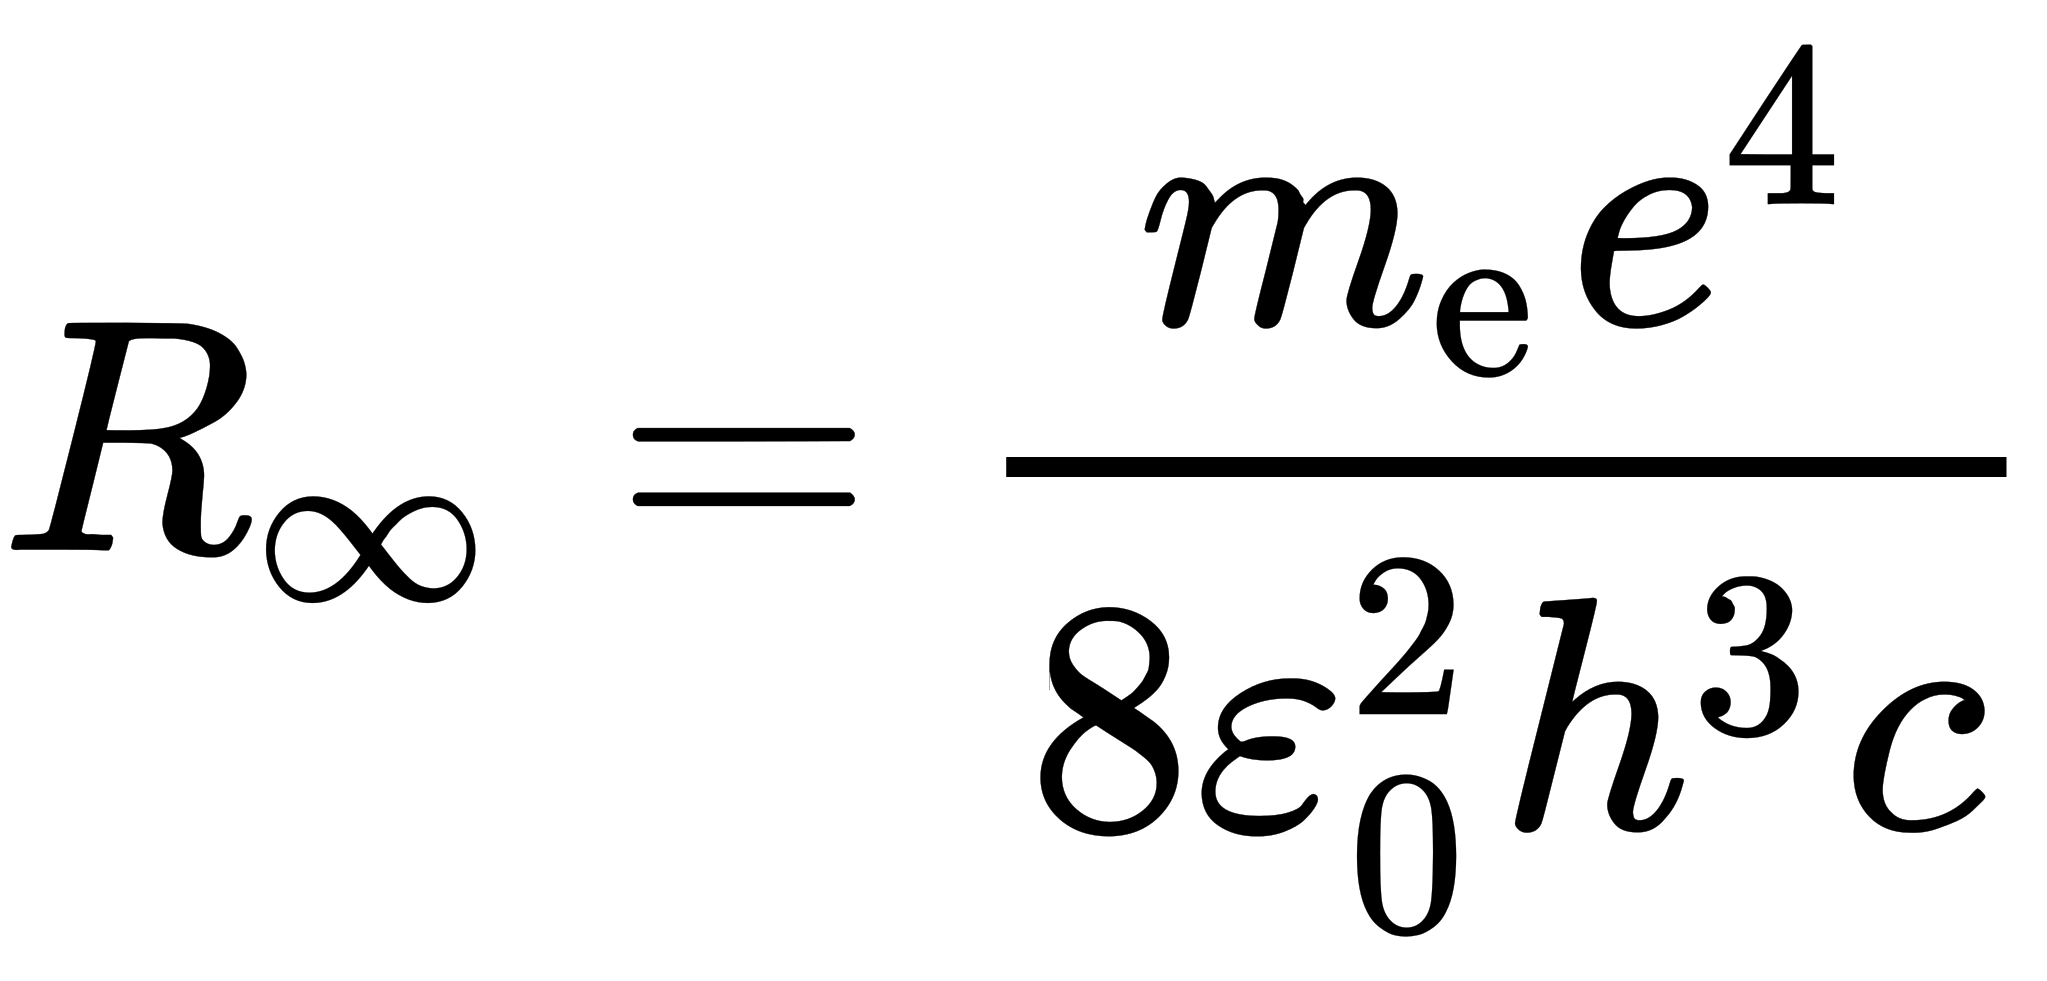
\includegraphics[width=0.45\linewidth]{img/1.png}
					\caption{A disconnected diagram which might contribute two point function. The principal part includes all the "real points" which are in the definition $\bra{\Omega} T{\phi(x)\phi(y)}\ket{\Omega}$, the bubble part contains no real points. }
				\end{figure}
			
			There are infinitely many diagrams that could replcae bubble subdiagram, see figure 2.
			\item What's the relationship between Feynman diagrams and S-matrix elements? Just a brief and clear answer. [Peskin goes absolutely rigorously and crazily through defining S-matrix via gaussian-wavepackets. I think it's even OK to miss this part of Peskin even for the first time.]
			\begin{figure}[H]
				\centering
				\includegraphics[width=0.9\linewidth]{img/2.png}
				\caption{Bubble diagrams. }
			\end{figure}
			\end{enumerate}
		\end{problem}
	\item
	\begin{problem}{\points[Peskin 4.4 and 4.8 / Schwartz 13]{}}
		\textbf{QED and $\phi^4$ Feynman Diagrams:}
	\end{problem}
	
	\noindent
	The final part of this problem is devoted to Feynman diagrams of two important theories. We will return to these rules throughout the course, since we are mostly deal with loops in this course. If you've not covered these materials, please read the specified chapters of Peskin to prepare yourself.
	\begin{enumerate}
		\item Write the momentum space Feynman diagrams for $\phi^4$ theory, these rules will guide us how to write the amplitude of a big Feynman diagram later on.
		\item Write the momentum space Feynman diagrams for QED theory. The Lagrangian is $\mathscr{L} = -\frac14 F_{\mu\nu}^2 +\bar{\psi}(i\gamma^\mu \partial_\mu -m)\psi -e\bar{\psi} \gamma^\mu \psi A_\mu$.
		\item Now write the amplitude for some diagrams in both theories:
			\begin{figure}[H]
				\centering
				\includegraphics[width=0.7\linewidth]{img/diag.png}
				\caption{The above diagrams correspond to $\phi^4$ theory, the below one correspond to QED.}
			\end{figure}
	\end{enumerate}
\end{enumerate}



\newpage

\section*{Problem 2: Quantum Mechanics Path Integral }
\begin{problem}
	We start this course by path integral, and it would be beneficial to have a minimal knowlege about the related concepts. Path integrals in field theory are generalizations of path integral in quantum mechanics. We explore the most important problem of the physics, which is the harmonic oscillator, and gain valuable lessons for our future\footnote{Notice that there are many mathematical subtlties [even ambiguities] with the definition of path integral. As a physics student, I found it more instructive to lay some fundations, and avoid asking highly sophisticated math-related questions about path integrals. Since these fascinating questions would not provide us with many physical intuition or concepts, but rather would indulge our mathematical curiosity. I can provide you with more examples in the classroom, but as a fact, only $\phi^4$ theory in four-dimensional spacetime has well-defined and rigorous path integral in the mathematical sense. To a mathematician, fermionic path integral is nothing more that a joke!}.
\end{problem}	

	\begin{enumerate}
	\item
	\begin{problem}{\points[Schwartz 14]{-}}
		\textbf{Intuition:} 
		
		\noindent
		The idea behind path integral is quite elementary, please express the idea based on what you could understand from the figure 4.
		\begin{figure}[H]
			\centering
			\includegraphics[width=0.7\linewidth]{img/pi1.png}
			\caption{Intuition regarding path integral in quantum mechanics.}
		\end{figure}
	\end{problem}
	\item
	\begin{problem}{\points[Sakurai 2.6]{-}}
		\textbf{Interpretation of path integral:}
		
		\noindent
		 Path integral could be seen as transition parobability is position space, breifly discuss why it's the case? You're expected to read the "Propagator as transition amplitude"‌ subsection and reepxress them.
		\noindent
	\end{problem}


	\item 
	\begin{problem}{\points{-}}
		\textbf{Gaussian Path Integrals:}
		
		\noindent
		A nice integral that appears in free-theories is the following,
		\[
		\underbrace{\int_{-\infty}^{+\infty} d \vec{x}}_{\int_{-\infty}^{\infty} dx_1\;\dots \;
		\int_{-\infty}^{\infty} dx_n
		} e^{-\frac12 \vec{x}^T \mathbf{A} \vec{x} +\vec{J}^T\vec{x}} = \sqrt{\frac{(2\pi)^n}{det(\mathbf{A})}}e^{\frac12\vec{J}^T\mathbf{A}^{-1} \vec{J}}
		\]
		Where, $\mathbf{A}$ is a symmetric $n\times n$ matrix with stricly positive eigenvalues, $\vec{J}$ is a n-vector, and all integrations on $n$ variables are on $\mathbb{R}$.
		
		\noindent
		Prove the relation, the easiest way is to diagonalize $\mathbf{A}$ matrix and change variables of integration.
	\end{problem}


\end{enumerate}
\noindent
\\
\\
\textbf{More discussion:} That's interesting you can give quantum physics via classical physics. What happens to all concepts in traditional quantization? How time-ordered products come in? Where is Hilbert space? These are alluring questions that should be addressed in different quantization schemes.
\end{document}